\documentclass[11pt]{article}

\usepackage{graphicx}
\usepackage{fancyref}
\usepackage{fancyhdr}
\usepackage{natbib}
\usepackage{wrapfig}

\bibliographystyle{abbrvnat}

\title{Physics 426 - Turbulence Notes}
\author{Jody Klymak}

\begin{document}

\maketitle
\pagestyle{fancy}

\section{Introduction}

The study of turbulence is necessarily hampered by the fact that turbulence is
inherently strongly non-linear.  In the previous notes we saw that variance
grows at the most unstable wavenumber quickly, but it also cascades to higher
and lower wavenumbers.  This is due to those modes growing, but also due to the
fast-growing modes interacting with one another randomly and eventually tearing
each other apart into turbulence.  This is seen in detail in a numerical
simulation (\fref{fig:SmythEtAl05}) where only two vortices are created, but
they still interact with one another and create  homogeneous turbulence. 


\begin{figure}[hbtp]
  \begin{center}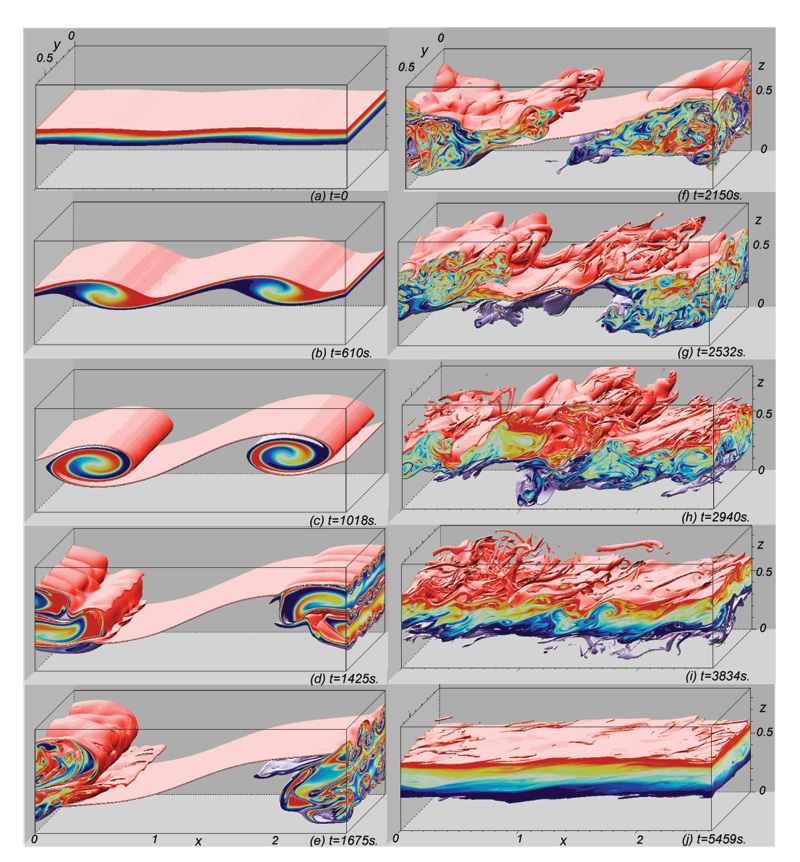
\includegraphics[width=5in]{images/SmythEtAl05}
    \caption{Numerical simulation \citep{smythetal05} of a shear isntability
transitioning to turbulence.}
    \label{fig:SmythEtAl05}
  \end{center}
\end{figure}

If the Reynolds number of the flow is great enough, the flow develops what we
call "homogeneous" turbulence, where the turbulent fluctuations stop carrying a
memory of the instability that formed them and they have universal statistical
properties.  

\section{Turbulent scales and spectra}

These universal statistical properties are often expressed as power spectra. 
So while we do not know what the velocity or value of any particular tracer is
at any time or place, we can characterize its variance as a function of
frequency and wavenumbers.  An example of this was shown in the previous write
up.   Another example is shown in \fref{fig:SmythMoum05Fig7} for the simulation
in \fref{fig:SmythEtAl05} and compared to observations.  

\begin{figure}[hbtp]
  \begin{center}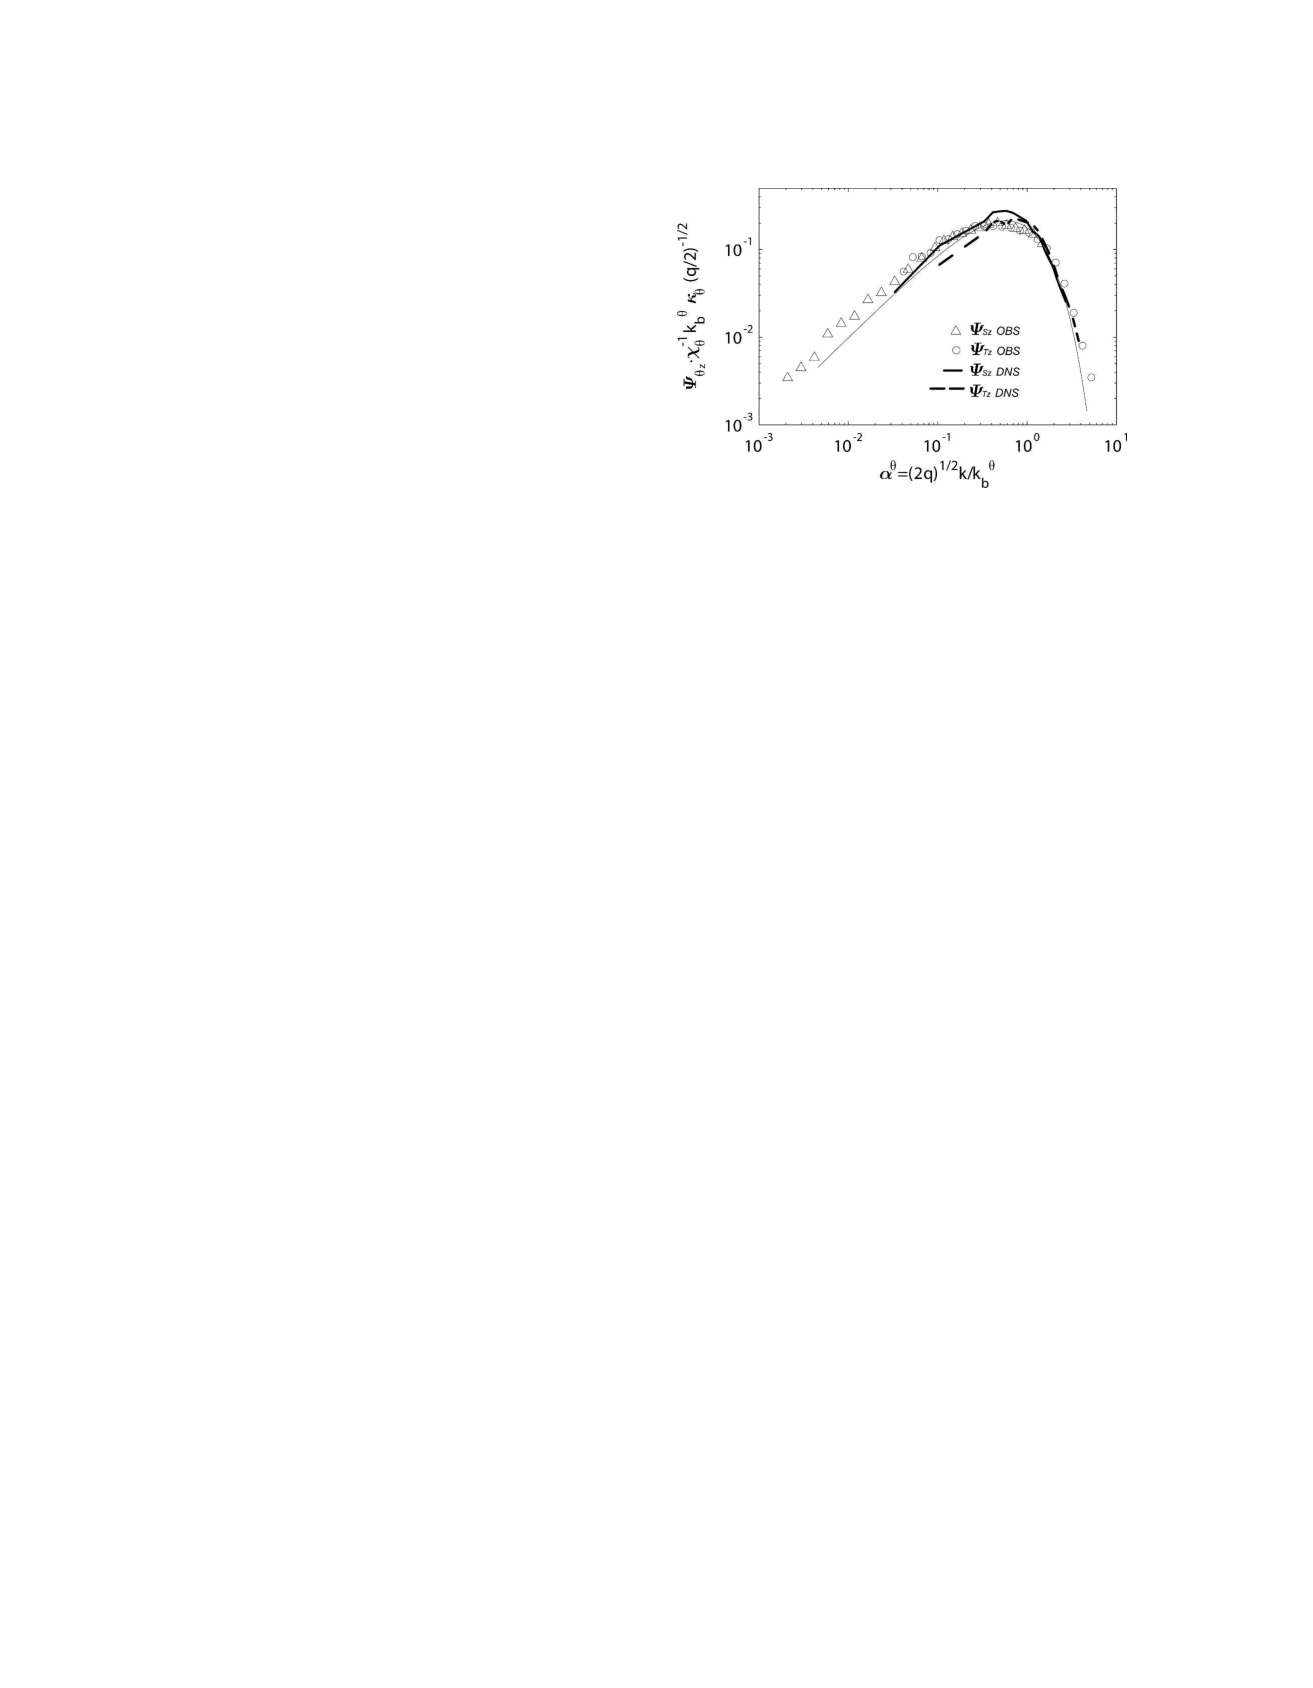
\includegraphics[width=3in]{images/SmythMoum05Fig7.pdf}
    \caption{Power spectra of tracer variance from \citep{smythetal05} compared
to oceanic observations of tracer spectra. The wavenumber $k$ has been scaled
to match a universal form}
    \label{fig:SmythMoum05Fig7}
  \end{center}
\end{figure}

This was of thinking about turbulence leads to a few very powerful, but
ultimately empirical results.  These results largely follow from dimensional
analysis which is surprisingly effective in this context.

\subsection[Kolmogrov scale]{Kolmogorov wavenumber and Inertial subrange}

First, it is important to determine the variables that are important to the
turbulence.  In steady state, the  rate that energy is put into the turbulence
is equal to the rate that it is removed, by viscous dissipation, which we
usually denote $\epsilon \ \mathrm{[m^2\,s^{-3}]}$.  The other variable that
sets the scale at which viscosity overcomes the turbulence is the strength of
the viscosity $\nu \ \mathrm{[m^2\, s^{-1}]}$.  These two variables combined
set the scale at which turbulent fluctuations die off, which we represent by a
wavenumber $k_{\nu} = \epsilon^{1/4}\nu^{-3/4}$.   This scale is small for most
flows and actually gets smaller as the strength of the turbulence ($\epsilon$)
increase.  In a turbulent channel in the waters near here,
$\epsilon\approx10^{-4}\ \mathrm{m^2\  s^{-3}}$ we get a value of $k_{s}
\approx 3000\ \mathrm{rad/m}$ or a length scale of 1 mm. This wavenumber,
$k_s$, is called the Kolmogorov wavenumber.   We can similarly use scaling
analysis to say that the shortest time scale of motion is $t_{\nu} \approx (\nu
/ \epsilon)^{1/2}$.  

This scaling works very well for predicting the scale at which turbulence
decays.  Measurements in Knight Inlet BC made by Ann Gargett (who is an
emeritus professor here) show that as the wavenumber approaches $k_s$ the power
spectrum of the velocity variance drops off rapidly
(\fref{fig:GargettEtal84Fig27}).  

\begin{figure}[hbtp]
  \begin{center}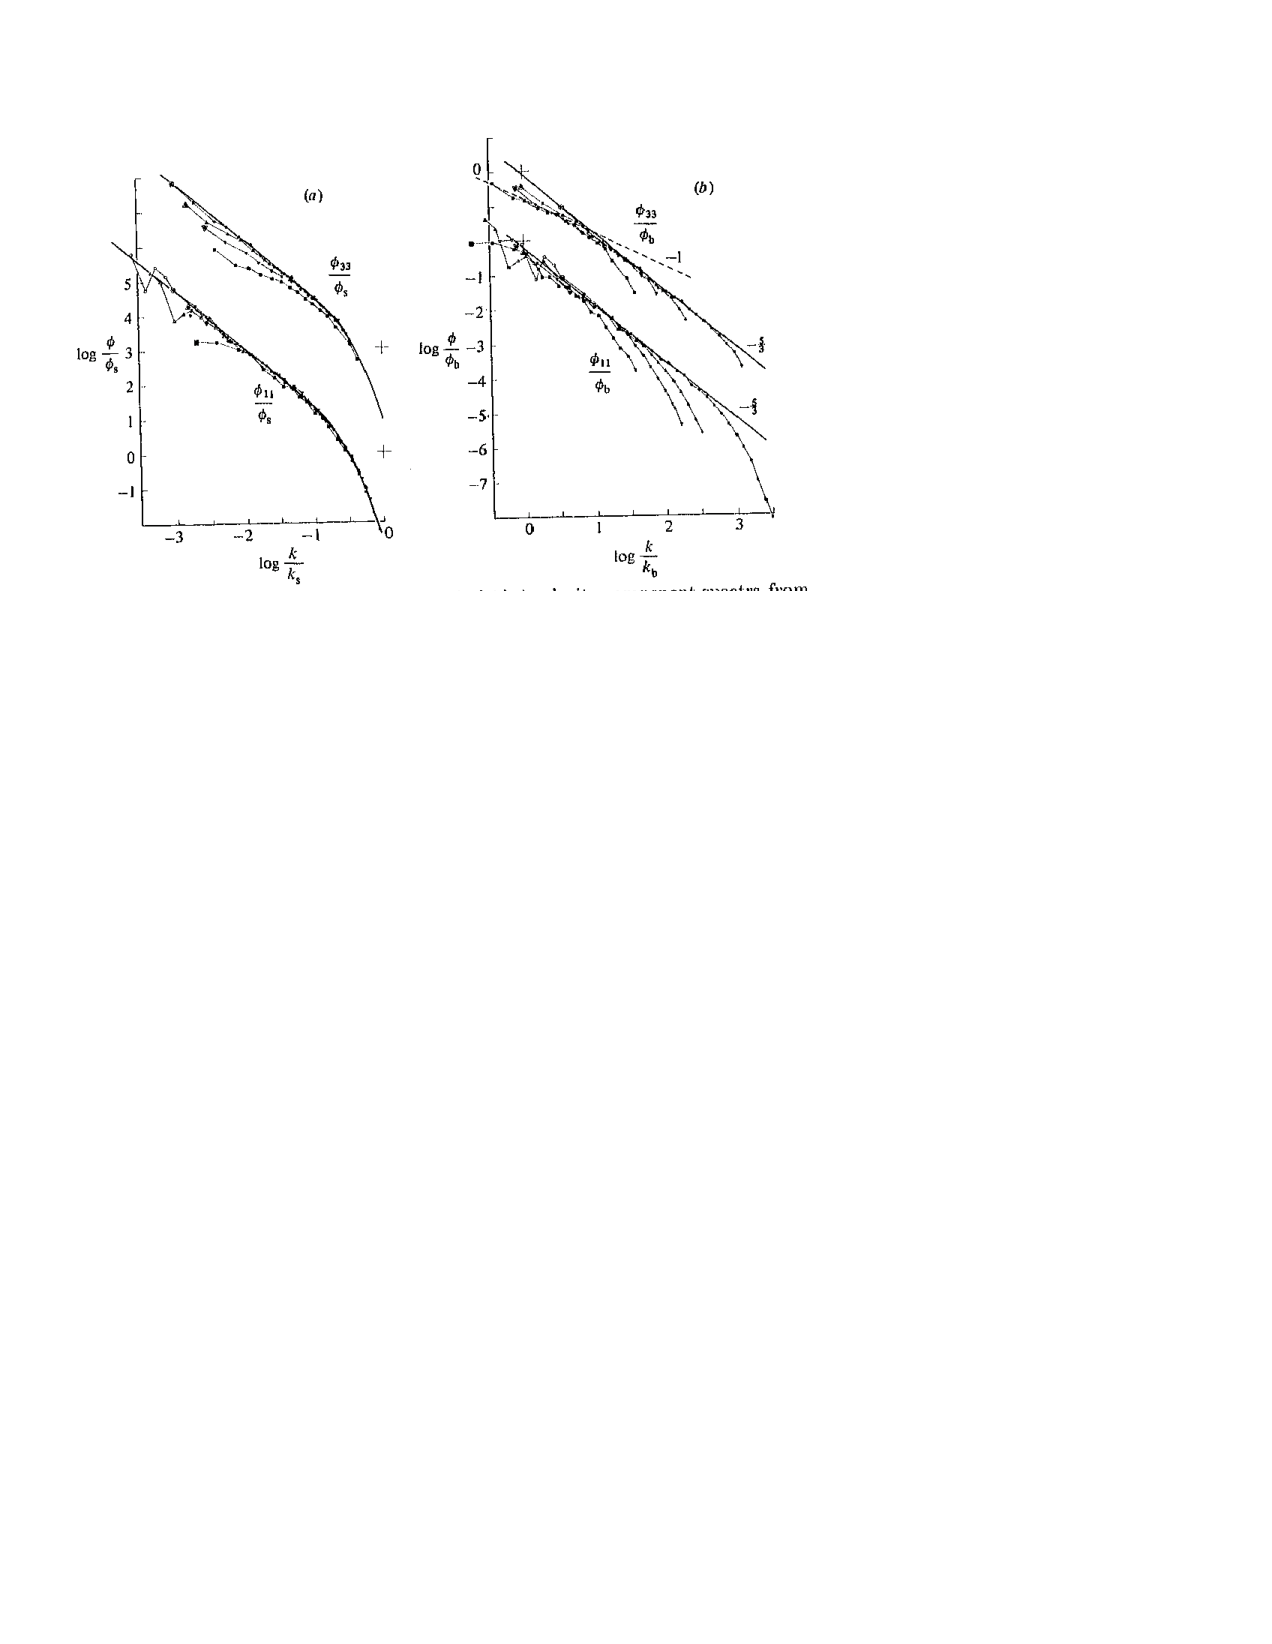
\includegraphics[width=4.5in]{images/GargettEtal84Fig27}     
  \caption{Power spectra of  a) velocity and b) tracer variance collected from
a submersible in Knight Inlet \citep{gargettetal84}.  In a) the horizontal
wavenumber is scaled by the Kolmogorov scale $k_s$.  In b) it is normalized by
the Batchelor wavenumber.}
    \label{fig:GargettEtal84Fig27}
  \end{center}
\end{figure}

It is also relatively clear that the spectra have a universal slope at lower
wavenumbers.  This region of wavenumber space between the viscous subrange and
the large scales at which energy in input is called the "inertial subrange". 
In this subrange, the spectrum only depends on the strength of the turbulence,
$\epsilon$ and the wavenumber $k$.  A velocity spectrum $\phi$ in wavenumber
space has units of $\mathrm{m^2s^{-2} / cpm}$ or $\mathrm{m^3\,s^{-2}}$, so
dimensional analysis says that $\phi \sim \epsilon^{2/3}k^{-5/3}$, and indeed
this is the slope of the spectra shown in \fref{fig:GargettEtal84Fig27}a. 


\subsection{Tracer subranges}

For a passive tracer, variance is destroyed at a rate $\chi\ \mathrm{[K^2
s^{-1}]}$, by diffusion $\kappa$ instead of viscosity.  For instance for heat,
variance is smoothed out by thermal diffusion.  In this case the smallest scale
of variance depends on three variables, $\epsilon$, $\nu$ and $\kappa$.  Since
$\kappa$ and $\nu$ have the same units we cannot appeal just to dimensional
analysis to determine the power laws, but instead consider that the Batchelor
scale is the scale at which the time to dissipate the energy at that scale is
equal to the time it takes to diffuse the variance away, yielding $k_b =
\epsilon^{1/4}\nu^{-1/4}\kappa^{-2/4}$.  

Hence for a tracer, we have a complicated situation where energy is put in at
large scales (\fref{fig:DillonCaldwell80aFig1}), there is an  "inertial
subrange" where both momentum and the tracer are stirred in tandem ($k<k_*$).
In this range $\phi_T\sim k^{-5/3}$, or in \fref{fig:DillonCaldwell80aFig1},
$\phi_ {dT/dz} \sim k^{1/3}$.   At some point viscosity becomes important, and
the power law changes to depend on $k$, $\epsilon$, $\chi$, \emph{and} $\nu$. 
These do not uniquely give the power law in the next subrange, called the
"viscous-convective" subrange, but it turns out that $\phi_T\sim k^{-1}$ (or
$\phi_ {dT/dz} \sim k^{1})$ as in \fref{fig:DillonCaldwell80aFig1}).  The third
subrange is the ``diffusive'' subrange where diffusivity finally becomes
important at the highest wavenumbers.  

\begin{figure}[hbtp]
  \begin{center}
    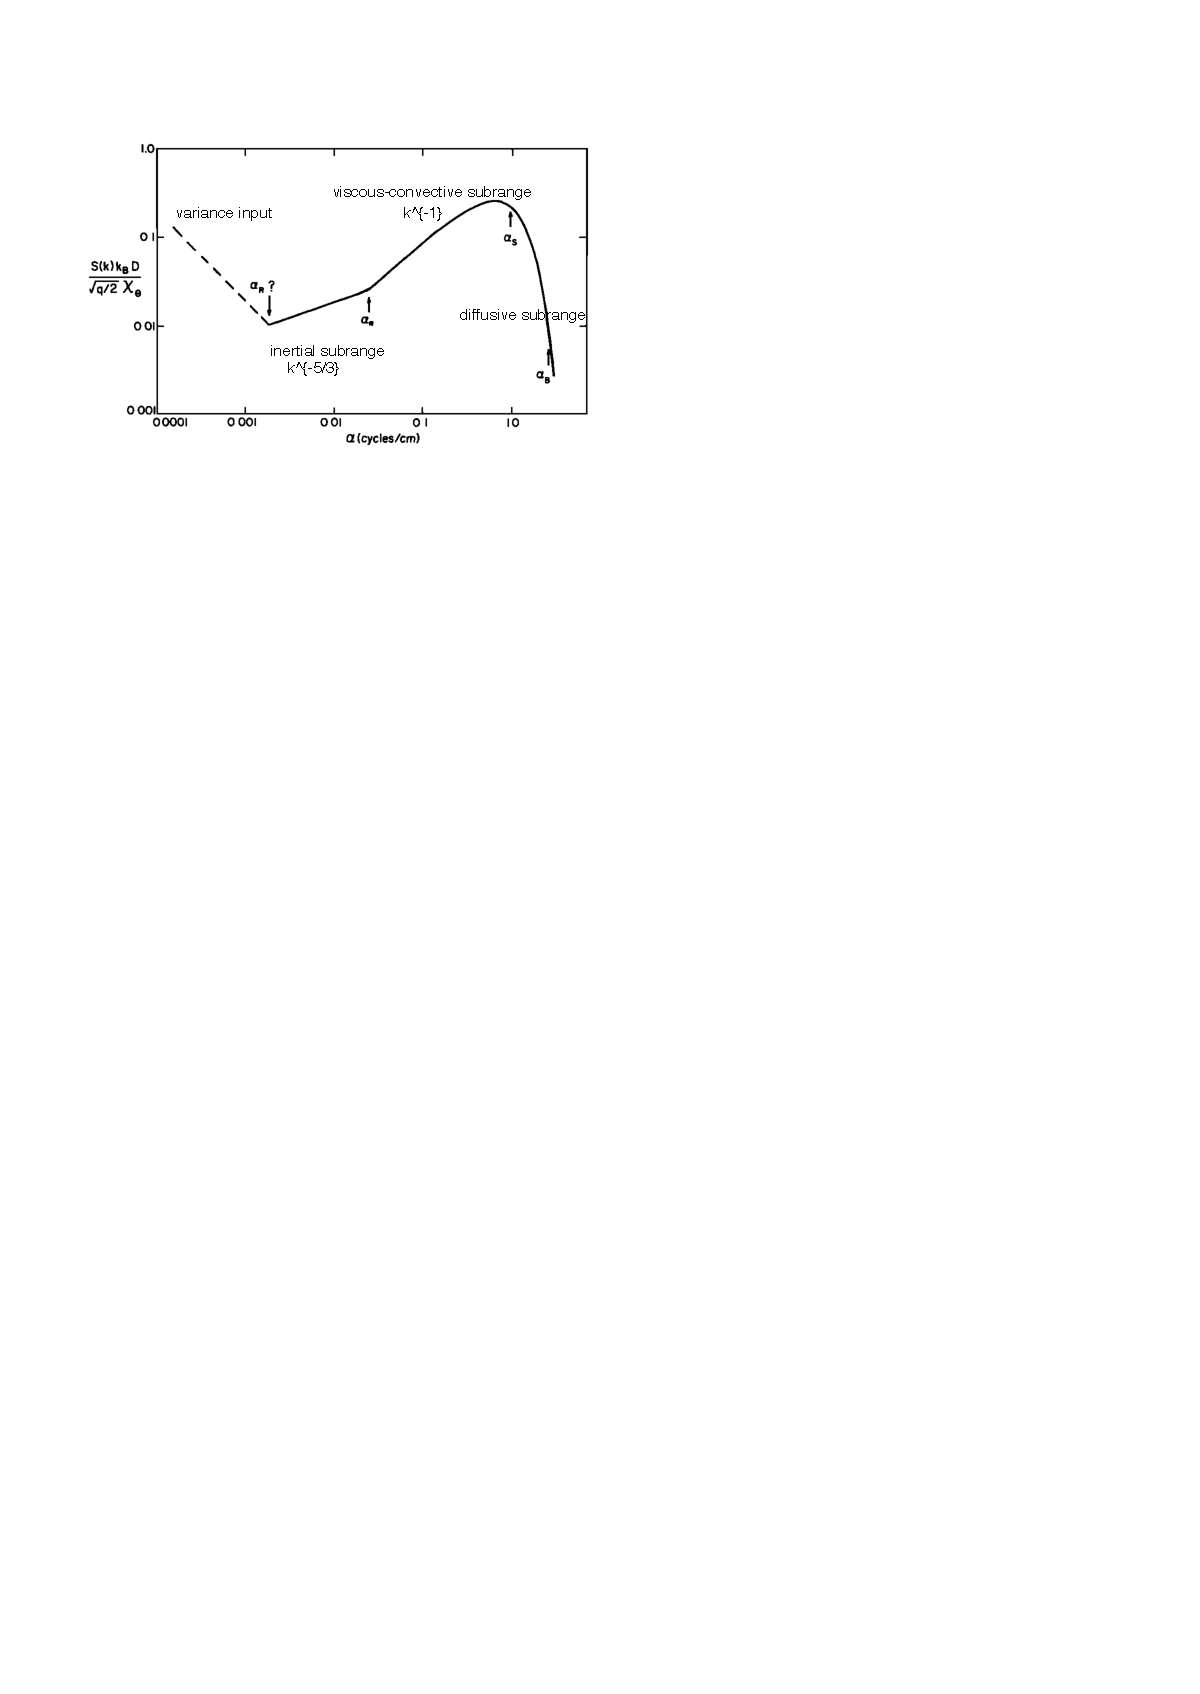
\includegraphics[width=5in]{images/DillonCaldwell80aFig1}
    \caption{Schematic temperature gradient spectrum \citep{dilloncaldwell80}. 
$\alpha_*$ is the scale to which momentum and tracer are stirred without the
effect of viscosity.  $\alpha_s$ is the Kolmogorov wavenumber, and $\alpha_B$
is the Batchelor wavenumber.}   
    \label{fig:DillonCaldwell80aFig1}
  \end{center}
\end{figure}

The universality of these spectral shapes is quite impressive for high-Reynolds
number flows, such as those found in the ocean \fref{fig:NashEtAl99Fig9},
though it is notoriously hard to observe the viscous subrange because it is so
small.  The measurements made in \fref{fig:NashEtAl99Fig9} are possibly using a
small-scale thermocouple, but this instrumentation is not very long lasting in
seawater.  

\begin{figure}[hbtp]
  \begin{center}
    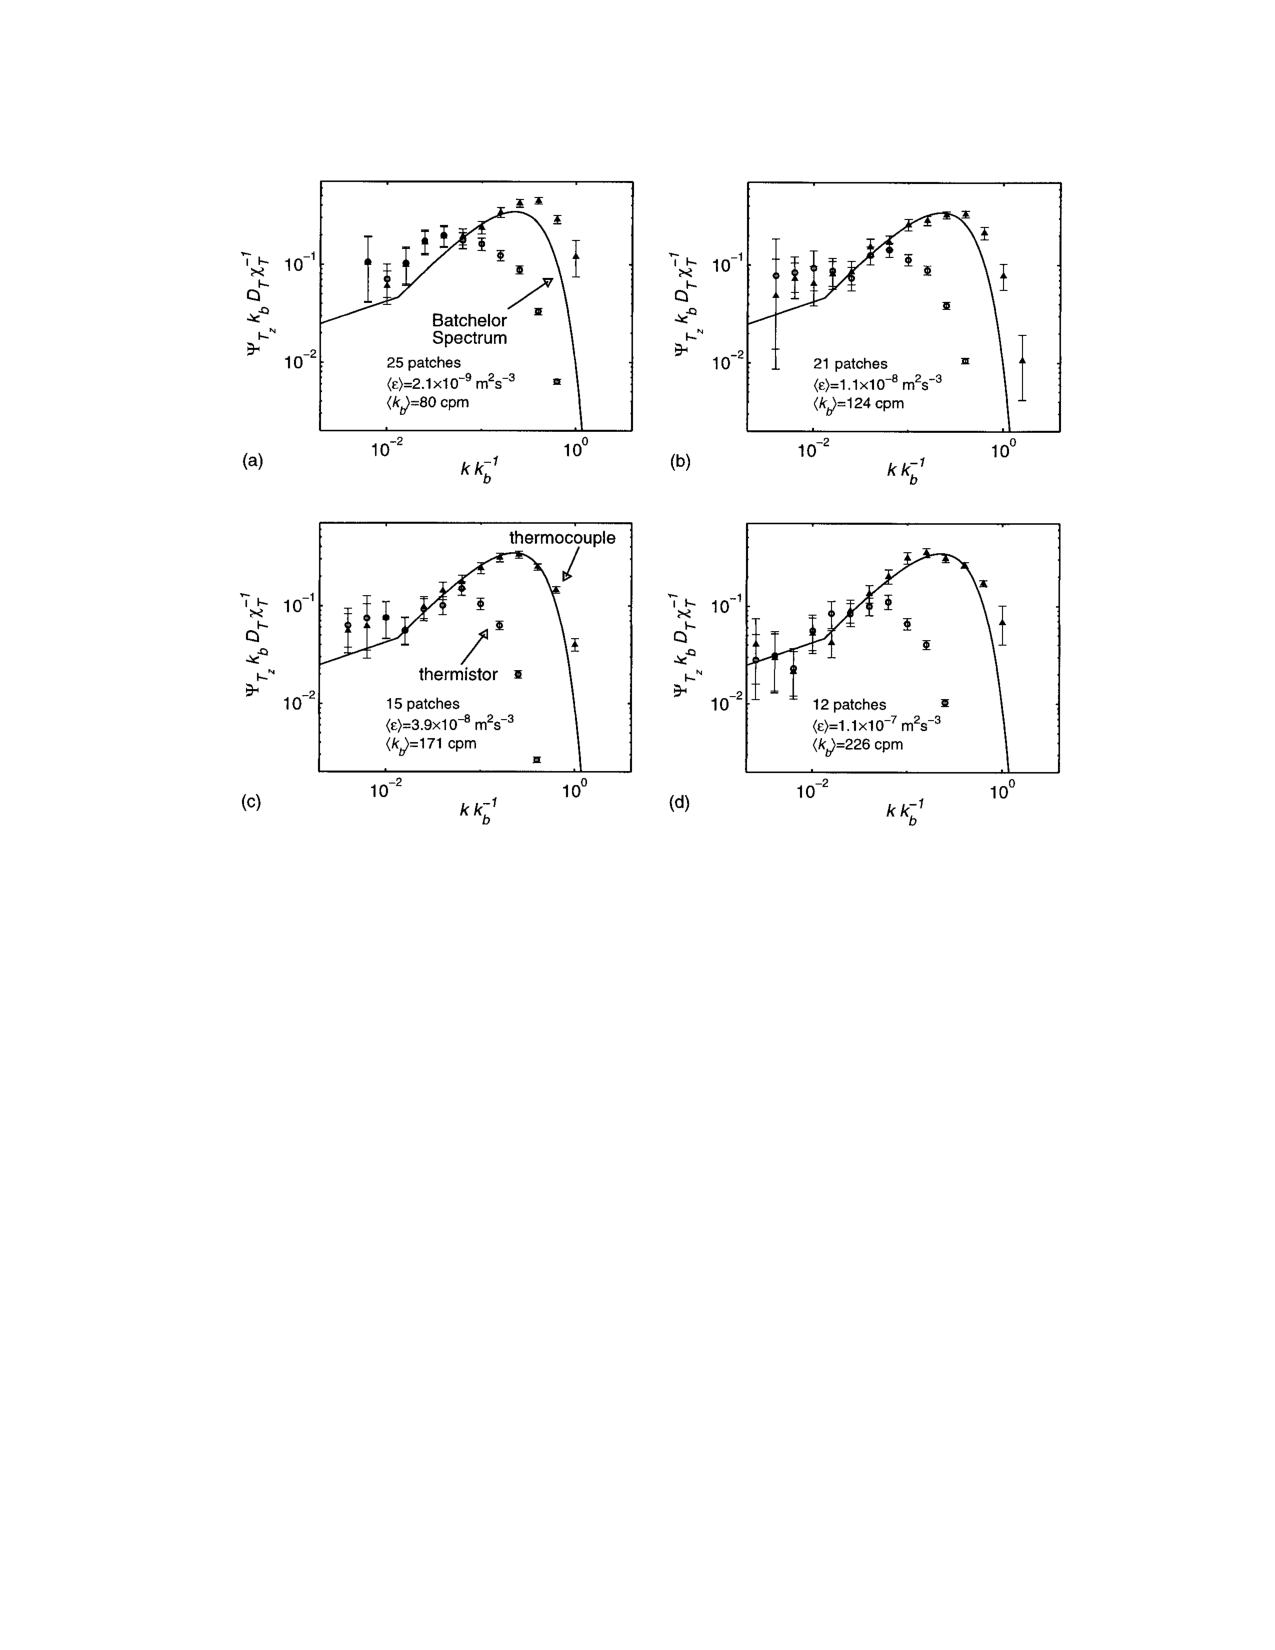
\includegraphics[width=5in]{images/NashEtAl99Fig9}
    \caption{Spectra of temperature gradient measured in the ocean using a
small-scale thermistor, and a smaller thermo-couple \citep{nashetal99}.  Note
the Batchelor scale is order 4 mm to 1 cm in these measurements, and it is very
hard to make measurements to such small scales.}   
    \label{fig:NashEtAl99Fig9}
  \end{center}
\end{figure}

As a note on the universality of the spectra - this has mostly only been shown
in geophysical flows where there is a large scale separation between the
Kolmogorov scale and/or Batchelor scale and the scale at which shear develops. 
For a small pipe, a few centimeters across, the Kolmogorov scale may be less
than an order of magnitude smaller than the pipe, and that may not be enough
"wavenumber space" for an inertial subrange to develop.  Hence the first
observations of these universal spectra were made in very energetic turbulence
in the ocean - the first such observation was made by \citet{grantetal62} based
out of DREP in Esquimalt by taking velocity measurements in Seymour Narrows
between Vancouver Island and Quadra Island.  

\subsection{Measuring turbulence}

Measuring turbulence is notoriously difficult. In the laboratory, it requires
small-scale velocity measurements.  Approaches include 
\begin{itemize}
  \item High-frequency acoustic  measurements that depend on the time-of-flight
of sound pulses or the Doppler effect on particles in the water. 
  \item Sheets of lasers on suspended particles in the fluid and video cameras
that track the motion of the particles in the sheets.  
  \item Temperature probes to measure small-scale fluctuations in temperature. 

\end{itemize}

Geophysical measurements are hard in that they often have trouble
contextualizing the flow that the turbulence is found in.  However, they have
the advantage that the turbulence is very strong, and hence the measurements
can be a bit cruder.  In the ocean, we either tow or profile vehicles
(\fref{fig:KlymakNash09Fig3}) equipped with shear probes and high-speed
thermistors (\fref{fig:KlymakNash09Fig5}).  An example from my thesis exhibits
some of the challenges with these methods (\fref{fig:KlymakGregg04Fig6}). 
These are measurements from Knight Inlet, with strong stratified tidal flow
over an underwater sill.  Collected with a vertical profiling instrument, the
data collection is sparse compared to the size of the flow, and multiple repeat
passes over the sill necessary to characterize the flow.  However, the flow is
constantly changing over the 12.4-h tidal cycle, so even these snapshots are
fragmentary.  

\begin{figure}[hbtp]
  \begin{center}
    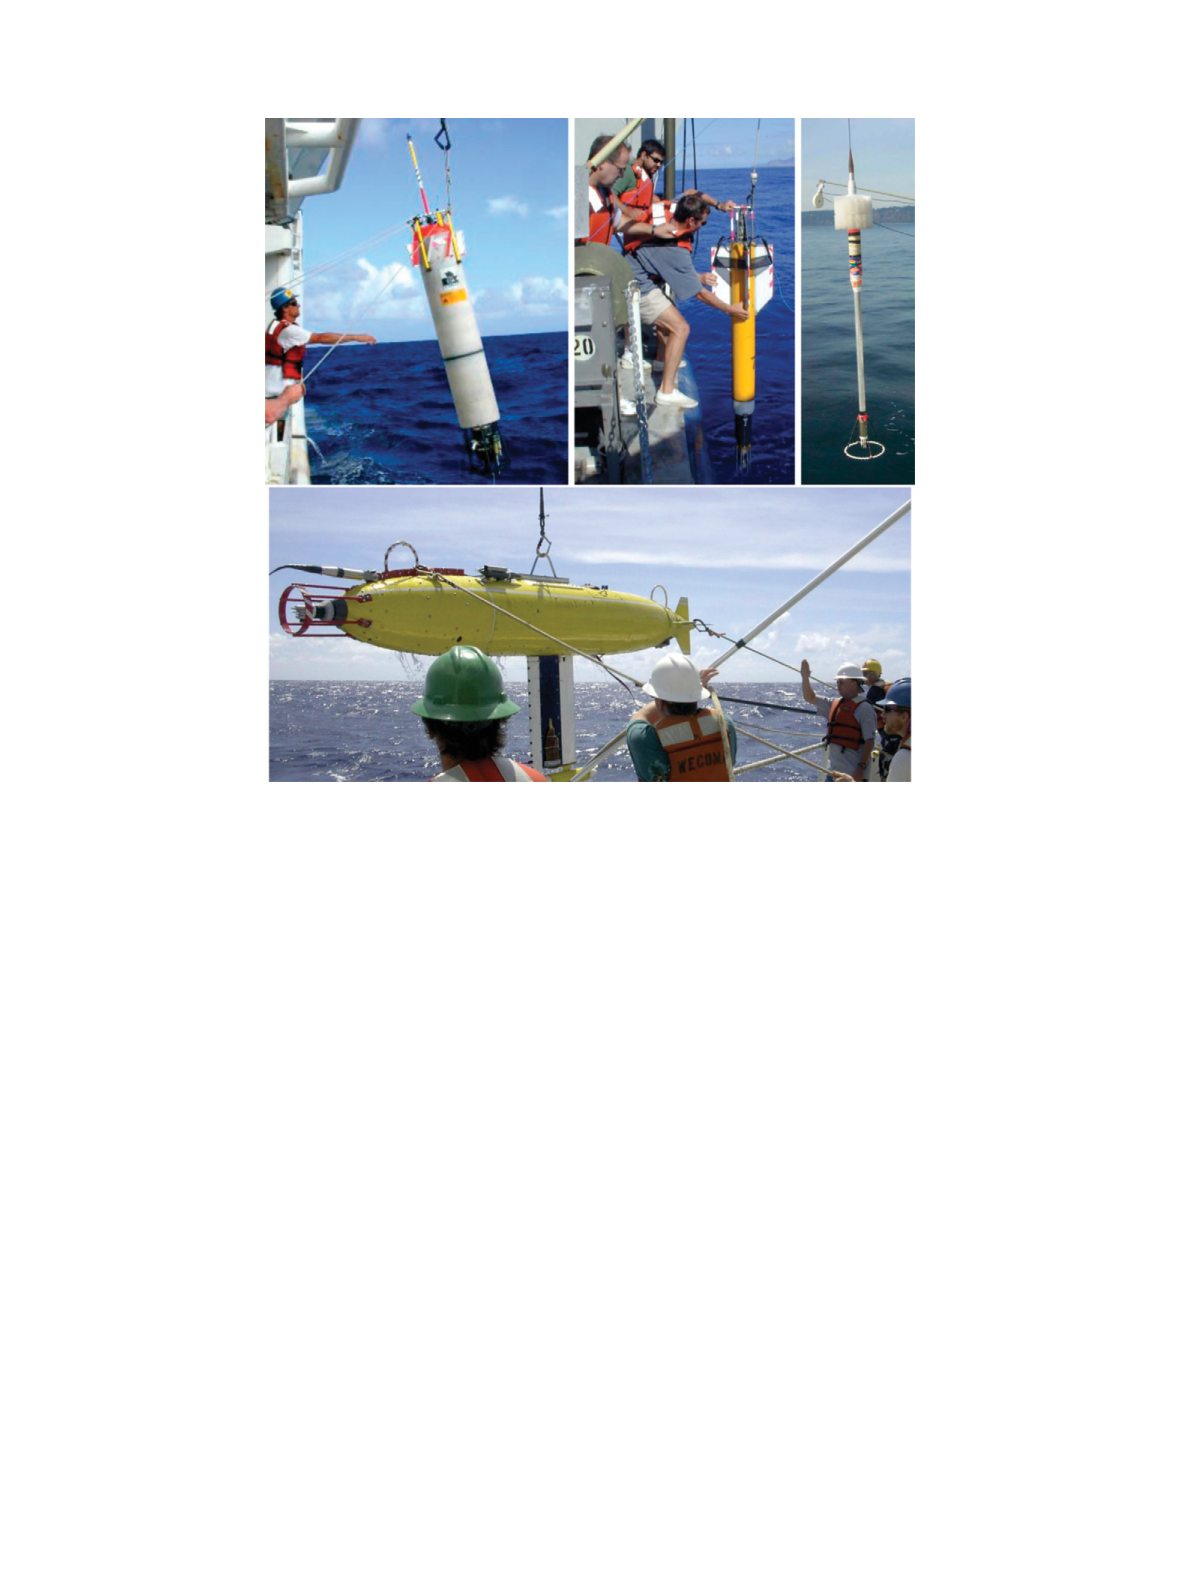
\includegraphics[width=4in]{images/KlymakNash09Fig3}
    \caption{Oceanic vehicles for measuring ocean turbulence
\citep{klymaknash09}. The upper three are vertical profilers that fall freely
from a ship.  The bottom is a towed instrument, similar to that used by
\citet{grantetal62, gargettetal84}.}   
    \label{fig:KlymakNash09Fig3}
  \end{center}
\end{figure}

\begin{figure}[hbtp]
  \begin{center}
    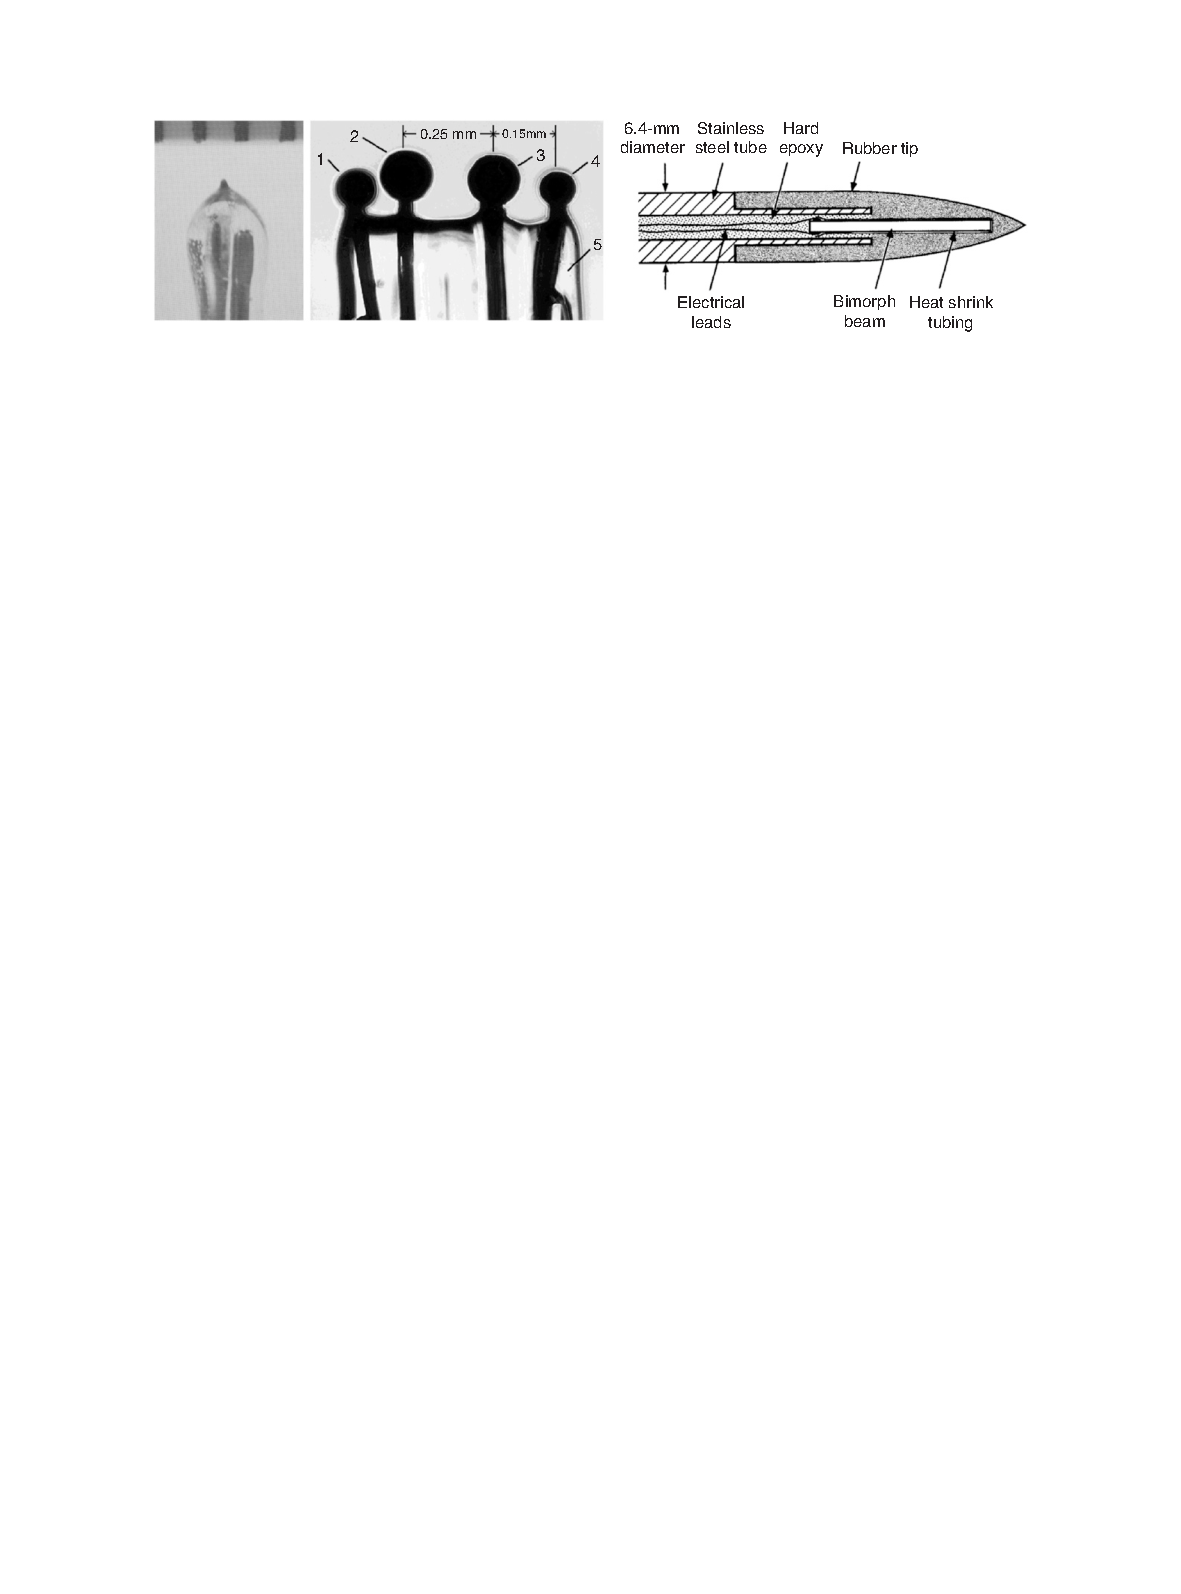
\includegraphics[width=4in]{images/KlymakNash09Fig5}
    \caption{Probes for measuring ocean turbulence \citep{klymaknash09}.  Left,
a fine-scale thermistor, a (fragile) microconductivity probe (with two anodes
and two electrodes), and a piezo-electric shear probe.}   
    \label{fig:KlymakNash09Fig5}
  \end{center}
\end{figure}


\begin{figure}[hbtp]
  \begin{center}
    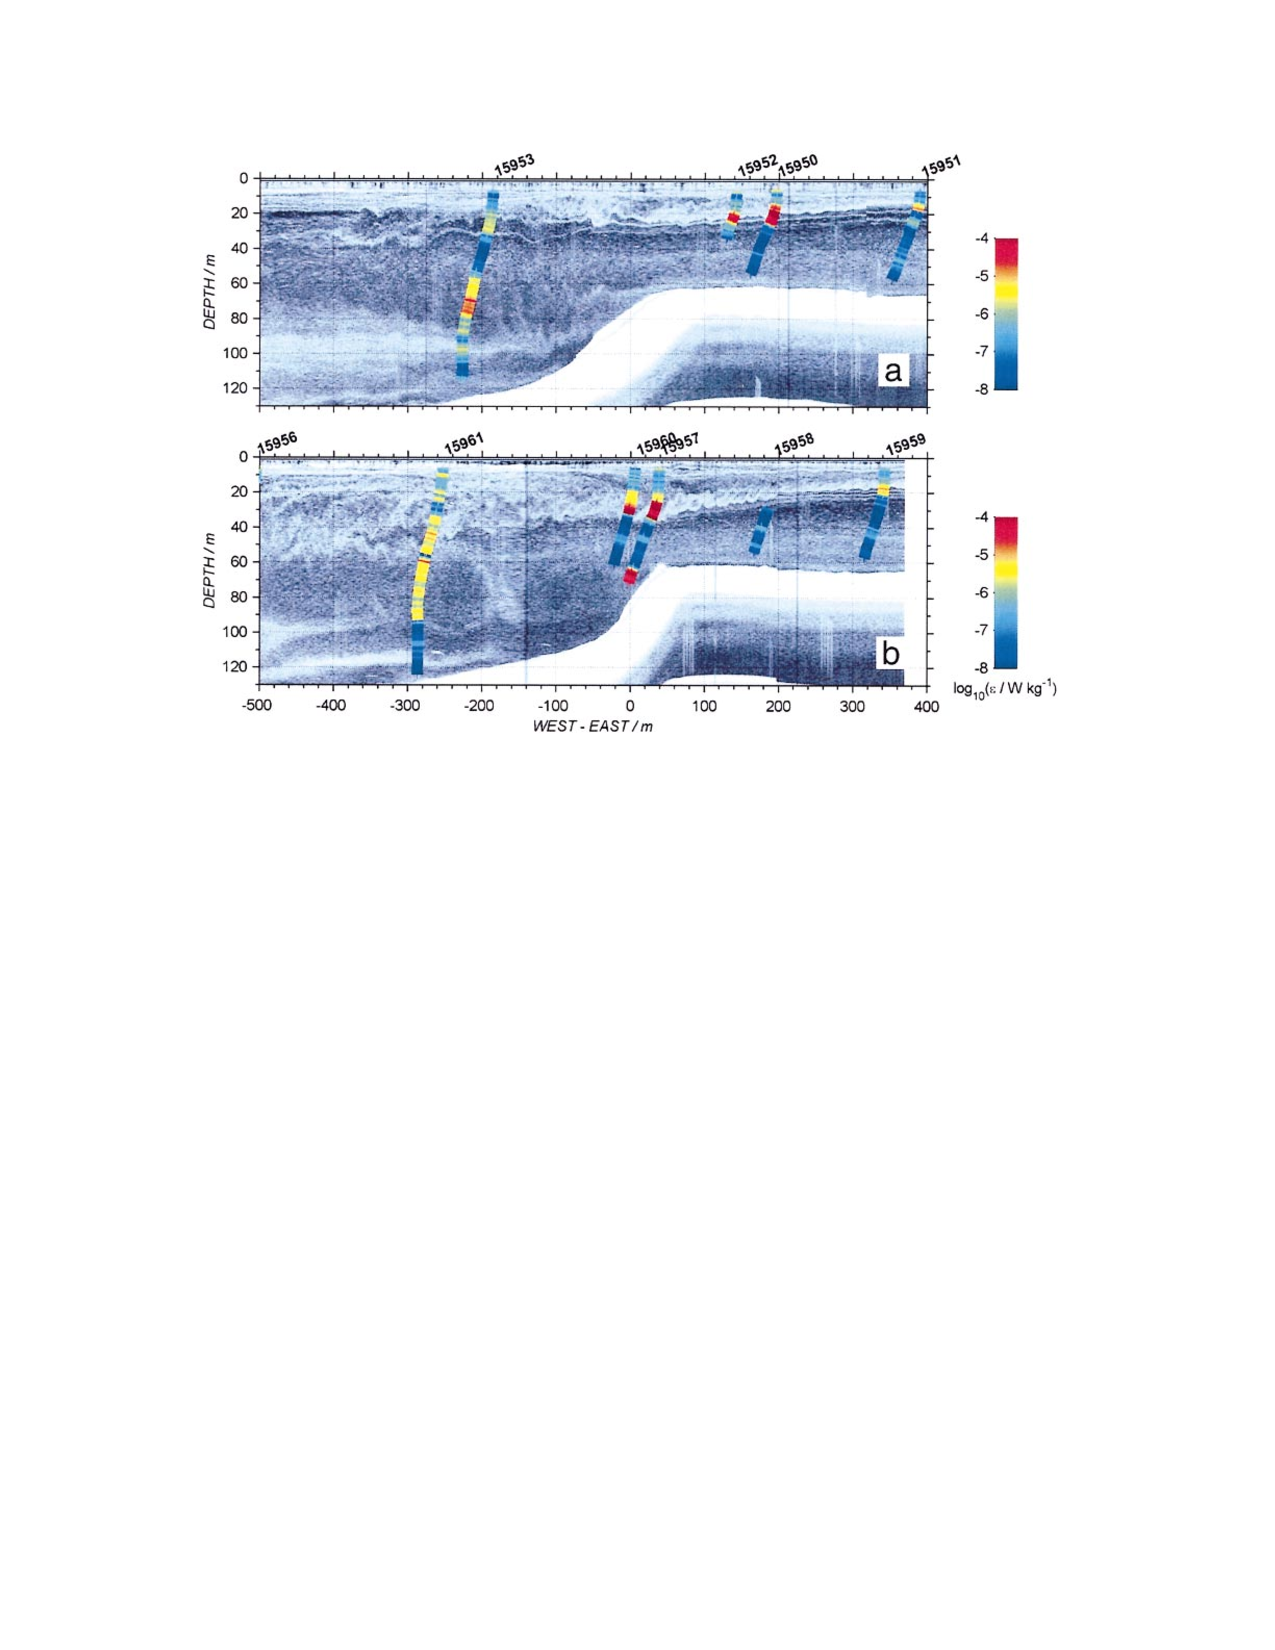
\includegraphics[width=5in]{images/KlymakGregg04Fig6}
    \caption{Turbulence measured from a turbulence profiler deployed in Knight
Inlet \citep{klymakgregg04}.  Flow is visualized using high-frequency acoustics
scattering off both biology (zooplankton) and sharp gradients in salt caused by
turbulence (and of course the seafloor).  The colored tracks are turbulence
dissipation rates measured by the profiler.  The flow is from right to left,
and is blocked  by the sill creating a hydraulic flow similar to the ones
studied in class.}   
    \label{fig:KlymakGregg04Fig6}
  \end{center}
\end{figure}

\clearpage
\section{Turbulent fluxes}

Turbulence leads to much faster diffusion of momentum and tracers.  Ultimately,
mixing of momentum and tracers must occur at the molecular level on scales that
are quite small.   Turbulence stirs the fluid and greatly increases the area
over  which molecular diffusion acts, as well as acting to sharpen gradients
which also increases turbulence fluxes (\fref{fig:SmythMoum01Schematic}).  

The approach we use to quantify this extra mixing is at its heart empirical. 
However, some important quantities in this empirical exercise can be derived if
we divide the flow into "mean" and "fluctuating" components in a procedure
known as "Reynolds Averaging".  

\begin{figure}[hbtp]
  \begin{center}
    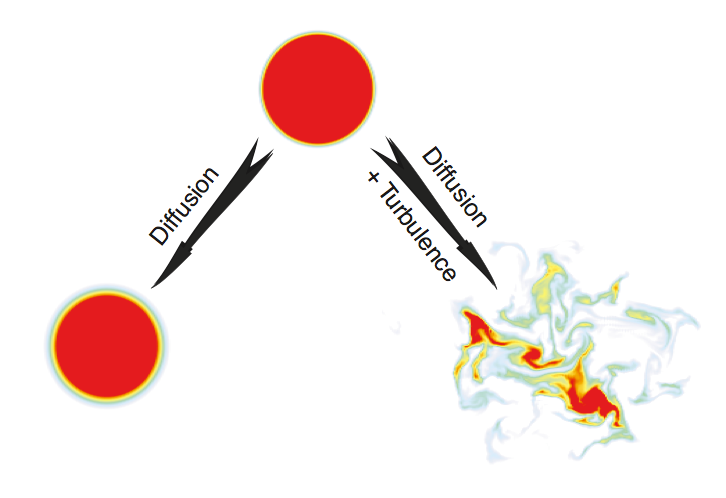
\includegraphics[width=3.5in]{images/SmythMoum01Schematic}
    \caption{Schematic of the importance of turbulence stirring to molecular
diffusion. }   
    \label{fig:SmythMoum01Schematic}
  \end{center}
\end{figure}

Here we write the equations of motion and decompose into a mean component and a
fluctuating component (denoted with primes).  For reference, the full equations
of motion, including a buoyancy term due to the temperature of the water are:
 \begin{eqnarray*}
     \frac{\partial \mathbf{\tilde{u}}}{\partial t} + \mathbf{\tilde{u}}\cdot
\nabla \mathbf{\tilde{u}} & = & -\frac{1}{\rho} \nabla \tilde{p} - g \left[  1
- \alpha(\tilde{T}-T_0)\right]\mathbf{k} + \nu \nabla^2 \mathbf{\tilde{u}}\\
     \nabla\cdot\mathbf{\tilde{u}} & = & 0\\
     \frac{\partial \tilde{T}}{\partial t} + \mathbf{\tilde{u}}\cdot\nabla
\tilde{T} & = & \kappa \nabla^2 \tilde{T}
 \end{eqnarray*}
where we have included a buoyancy term in the z momentum equation and $\alpha$
is a "thermal expansion" co-efficient that is linear around $T_0$.  

The Reynolds decomposition is to then say
\begin{eqnarray*}
    \mathbf{\tilde{u}} & = & \mathbf{U} + \mathbf{u'}\\
    \tilde{p} & = & P + p'\\
    \tilde{T} & = & T + T'\\
\end{eqnarray*}
where over some spatial or temporal interval the turbulent quantities are zero:
$\overline{\mathbf{u'}} = \overline{p'} = \overline{T'} = 0$.  

These are then substituted into the equations of motion:
\begin{eqnarray*}
     \frac{\partial (\mathbf{u}+\mathbf{U})}{\partial t} +
(\mathbf{u}+\mathbf{U})\cdot \nabla (\mathbf{u}+\mathbf{U}) & = &
-\frac{1}{\rho} \nabla (P+p') - g \left[  1 - \alpha(T+T'-T_0)\right]\mathbf{k}
+ \nu \nabla^2(\mathbf{u}+\mathbf{U})\\
     \nabla\cdot\mathbf{(\mathbf{u}+\mathbf{U})} & = & 0\\
     \frac{\partial (T+T')}{\partial t} +
\mathbf{(\mathbf{u}+\mathbf{U})}\cdot\nabla (T+T') & = & \kappa \nabla^2
(T+T')
 \end{eqnarray*}
And then we take the same average that defined the Reynolds decomposition. 
i.e. for the continuity equation:

\begin{equation}
    \overline{\nabla\cdot\mathbf{(\mathbf{u}+\mathbf{U})}} = \nabla\cdot
\mathbf{U} + \overline{\nabla\cdot \mathbf{u}}  = 0
\end{equation}
But the second term averages to zero because $\overline{\nabla\cdot \mathbf{u}}
= \nabla\cdot \overline{\mathbf{u}} = 0$, so this means that
$\nabla\cdot\mathbf{U} = 0$.  Subtracting from the full continuity equation
this means that $\nabla\cdot \mathbf{u} = 0$ as well.  

The same procedure on the momentum equation yields an equation for the slowly
evolving flow of:
\begin{equation}
    \frac{\partial \mathbf{U}}{\partial t} + \mathbf{U}\cdot \nabla \mathbf{U}
+ \overline{\mathbf{u} \cdot \nabla \mathbf{u}} = -\frac{1}{\rho} \nabla P - g
\left[ 1 - \alpha \left( T-T_0 \right) \right] \mathbf{k} + \nu\nabla^2
\mathbf{U}
\end{equation}
where the only term that remains from the turbulent quantity is the quadratic
term in $\mathbf{u}$.  


The terms represented by  $\overline{\mathbf{u}\cdot\nabla \mathbf{u}}$ are the
turbulent stresses, as opposed to the viscous stresses that are encapsulated by
the last term.  This is the only place in this class where Einstein notation
would be very useful, but lets just write out the x-momentum terms of this
equation
\begin{eqnarray*}
    \overline{\mathbf{u}\cdot\nabla \mathbf{u}}\cdot\mathbf{i} & = &\overline{u
\frac{\partial}{\partial x} u} + \overline{v\frac{\partial}{\partial y} u} +
\overline{w\frac{\partial}{\partial z} u}  \\ & = &
\ \frac{\partial}{\partial x} \overline{u^2} + \frac{\partial}{\partial y}
\overline{u v} + \frac{\partial}{\partial z} \overline{uw} 
\end{eqnarray*}
and then we note the analogue to the viscous terms in the x-momentum equation:
\begin{eqnarray*}
    \nu\nabla^2 \mathbf{U}\cdot\mathrm{i} & = & \frac{\partial}{\partial
x}\left( \nu \frac{\partial U}{\partial x}\right) + \frac{\partial}{\partial
y}\left( \nu \frac{\partial U}{\partial y}\right) + \frac{\partial}{\partial
z}\left( \nu \frac{\partial U}{\partial z}\right) 
\end{eqnarray*}
where recall that we said the viscous stress transporting x-momentum in the
z-direction was $\tau_{xz} = -\nu\frac{\partial U}{\partial z}$.  So in direct
analogy, we say that $-\overline{uw}$ is the turbulent stress that carries
x-momentum in the z-direction.  Similarly $-\overline{uv}$ is turbulent stress
carrying x-momentum in the z-direction and $-\overline{u^2}$ is turbulent
stress carrying x-momentum in the x-direction.  

To better understand this transfer of momentum, consider a  flow in the
x-direction that is sheared in the vertical (\fref{fig:ReynoldsStress}).  If
there is a turbulent $w<0$ in the flow, it tends to bring faster water down
with it, meaning on average $u>0$, and hence $-\overline{uw} > 0$ and positive
x-momentum is transfered down.  Exactly the same direction of momentum transfer
happens if $w>0$ and transporting slower fluid up in the water column, and
hence the average of $-\overline{uw}$ is a "stress" on the flow seeking to
homogenize the momentum.  This is the same sense that the momentum is
homogenized molecularly by $\tau_{xz}$.  

\begin{figure}[hbtp]
  \begin{center}
    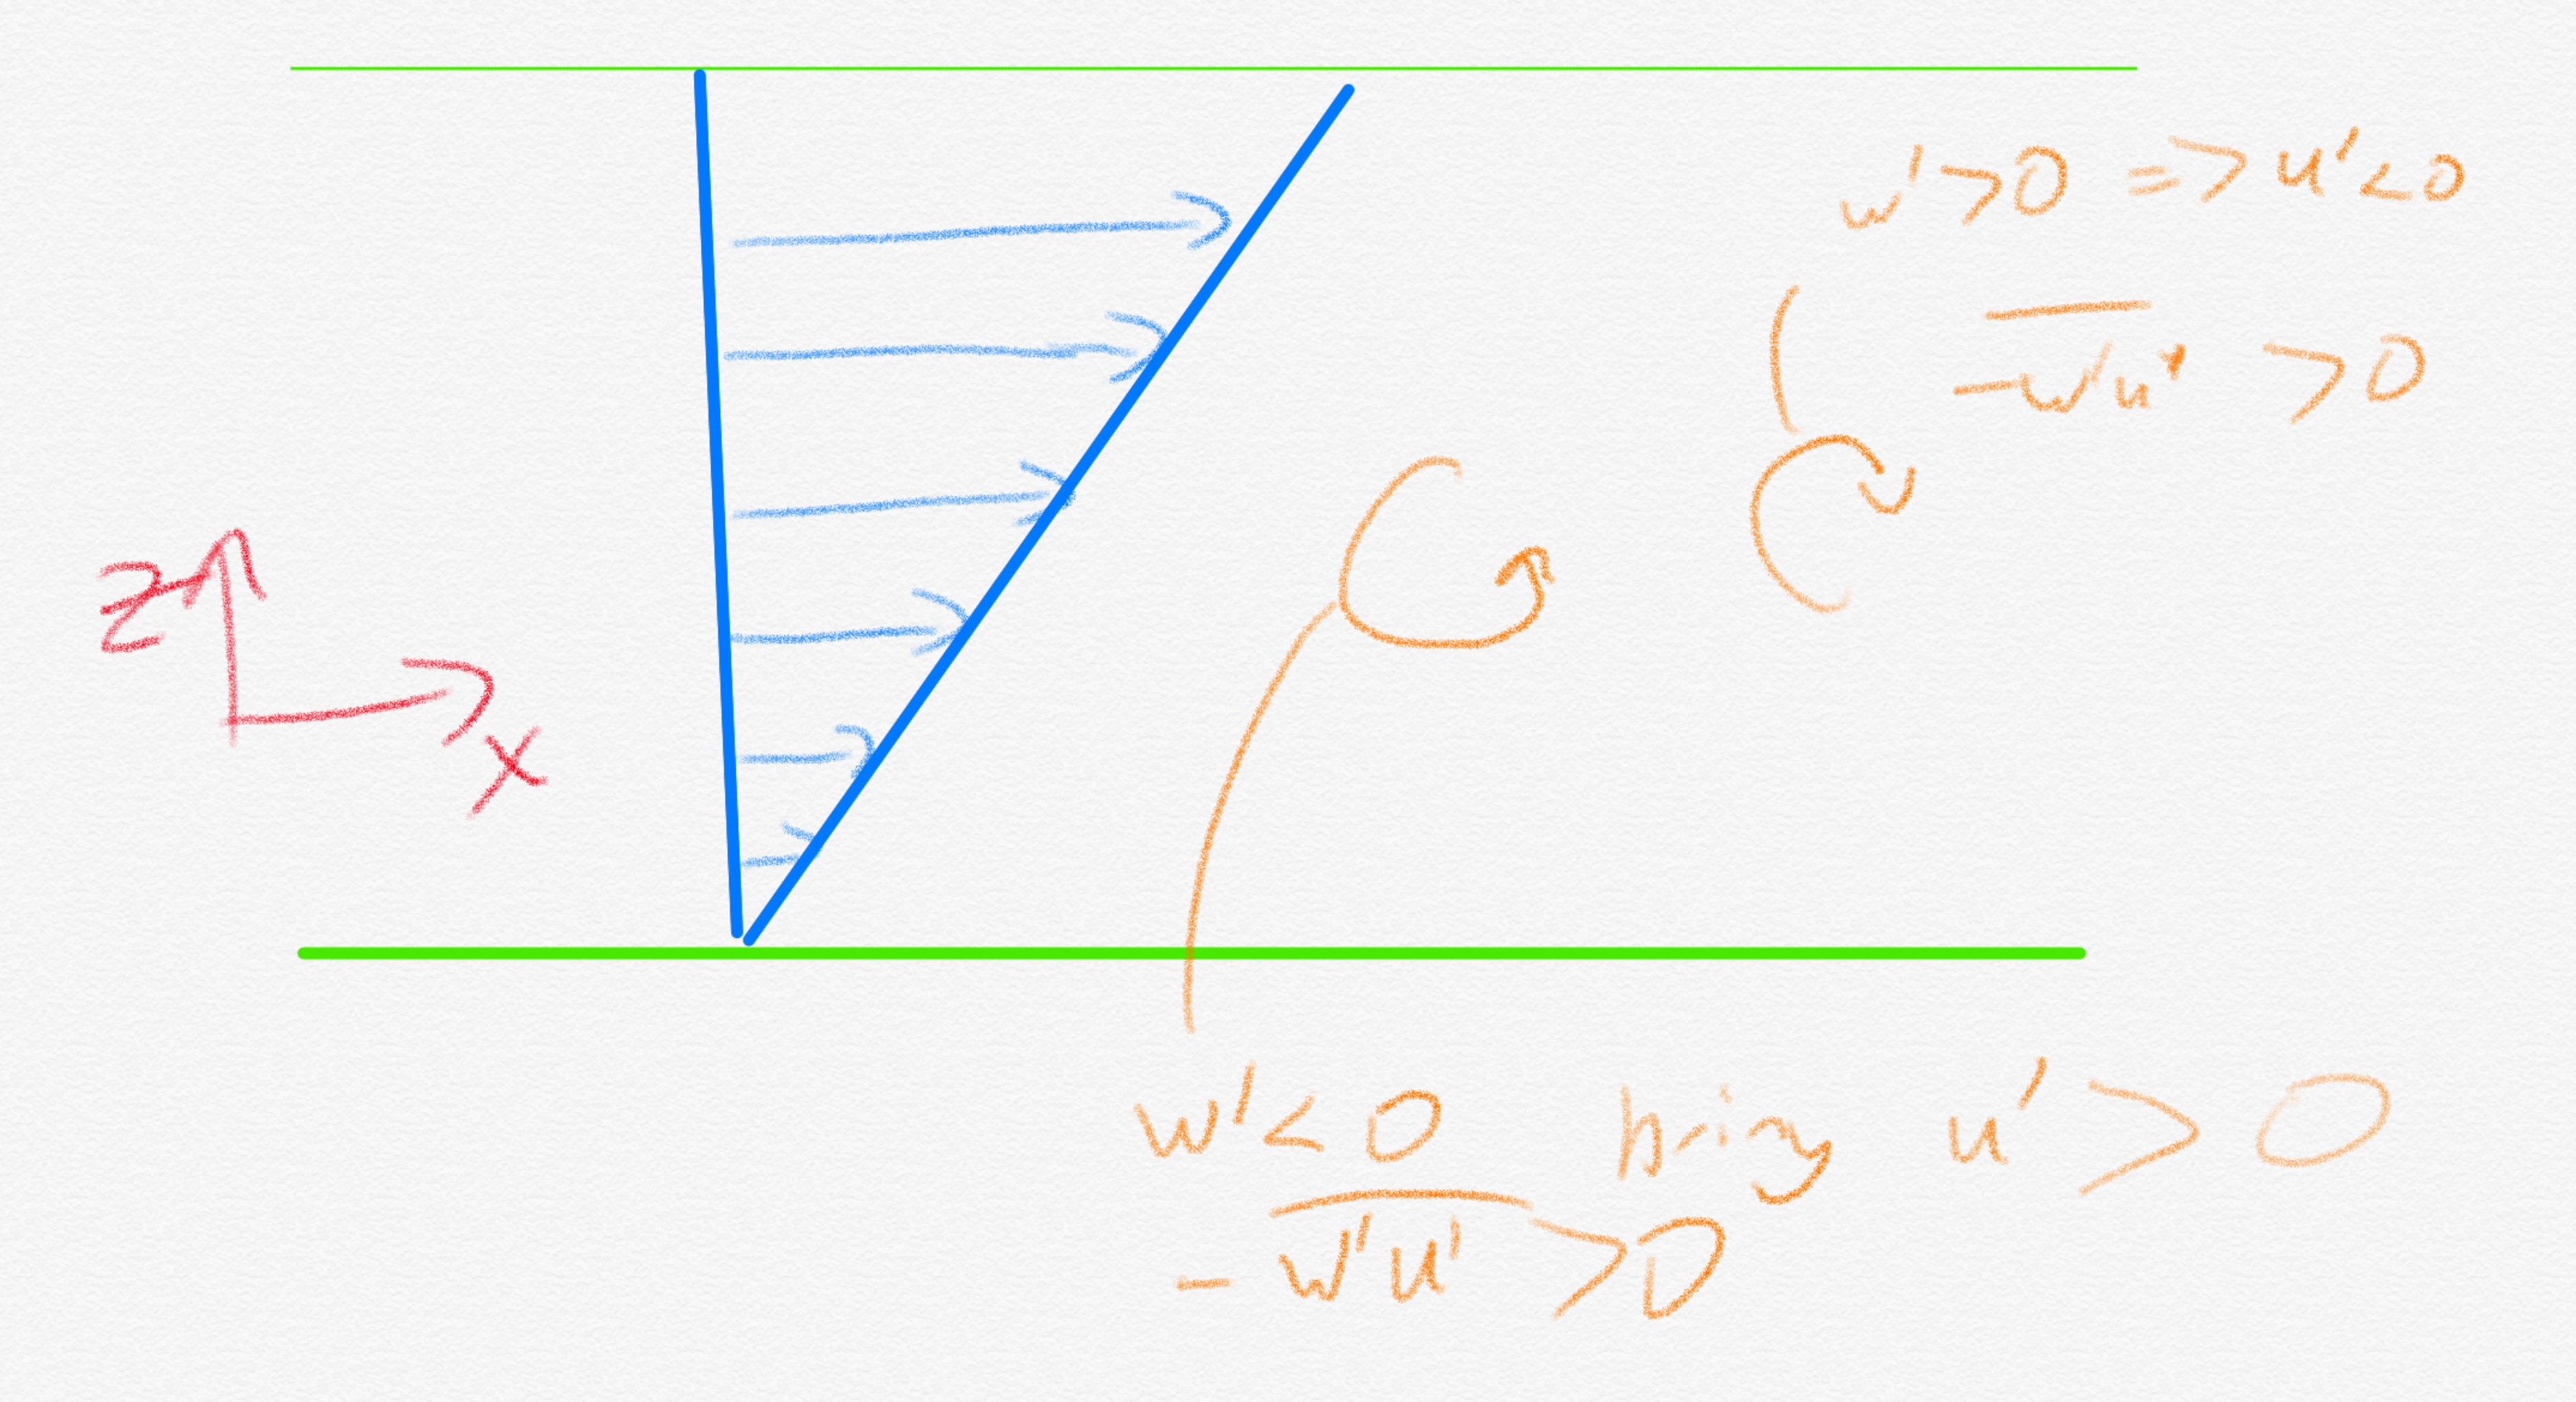
\includegraphics[width=5in]{images/ReynoldsStress}
    \caption{Sketch of sheared flow and the effect of positive and negative
fluctuations in $w'$ on the flow.}   
    \label{fig:ReynoldsStress}
  \end{center}
\end{figure}

Given the analogy with molecular viscous stress, its quite natural to seek a
parameterization of the turbulent stresses in terms of the large scale flow,
and indeed this is what is done in numerical simulations that cannot hope to
resolve the full spectrum of turbulence.  In the most general case we say
\begin{equation}
  \overline{\mathbf{u}\cdot \nabla \mathbf{u}} = \kappa_T \nabla^2 \mathbf{U}
\end{equation}
which is equivalent to saying that the turbulent stress is proportional to the
\emph{mean} shear. e.g.\ for the x-momentum equation:
\begin{equation}
  \overline{\mathbf{u}\cdot \nabla \mathbf{u}}\cdot \mathbf{i} = \kappa_T
\nabla^2 U
\end{equation}
In general $\kappa_T$ is \emph{much} larger than $\nu$ and the turbulent mixing
dominates the molecular.   The challenge, of course, is knowing what $\kappa_T$
should be.  This is an empirical and field-dependent endeavour, and is still a
topic of heavy research.  

\section{Notes on numerically simulating turbulent flows}

Turbulent flows are very hard to simulate numerically.  In 2020, a super-large
gigantic super computer cluster consists of 64k cores.  A good rule of thumb is
no more than domain sizes that as $64^3$ in size.  If we divide the 64k cores
evenly among all three directions, we get a domain size of $256k$ cells in each
direction.   If we are to resolve the Kolmogorov scale for moderately strong
turbulence of $\epsilon \sim 10^{-6}\ \mathrm{m^2s^{-3}}$, then $\eta =  1
\mathrm{mm}$ and our numerical simulation will extend 256 m in each direction. 
This would be a truly fabulous simulation but extremely expensive as we would
also have to resolve the CFL criteria of the flow.  In the ocean this is on the
order of 1 m/s, so our 1 mm grid cells would require timesteps of less than
0.001 s.  The problem worsens when the dissipation rate increases.  

Such expensive \emph{direct numerical simulations} (DNS) are not generally
carried out, and whenever DNS is applied usually much smaller domains are
considered (i.e.\ \fref{fig:SmythEtAl05}).  A less intensive method to
approximate turbulence is to suppose that the model resolves the big billows in
the instability, i.e.\ the roll-ups in \fref{fig:SmythEtAl05}, and then applies
an enhanced viscosity where it resolves strong shear.  The strength of this
enhanced viscosity does not matter too much because it generally just acts to
destroy whatever is caught in the roll-up.  This approach is called \emph{large
eddy simulation} (LES) and is naturally less precise than DNS, but only needs
resolution on the scale of the breaking eddies (say 10-s of cm) versus the
Kolmogorov scale (mm).  

Finally, there are even cruder parameterizations that apply when the simulation
cannot resolve the turbulent roll-ups.  For instance a global ocean simulation
will often be run at scales of 10-s of kilometers (or 100s) and will have no
hope of simulating shear instabilities, even relatively large ones like we
would find in large-scale lateral instabilities.  In these cases, turbulence is
usually estimated from large-scale shear $\partial U / \partial z$ and the
change of stratification $\partial \rho / \partial z$.  If the ratio of these
becomes too high, the flow is assumed to become turbulent and mixing is applied
until the ratio drops again.  In general this works fine to keep the model
running, but it will drift from observed conditions over longer time scales,
and hence the model usually needs to be nudged back to reality via assimilation
of observations.   


\bibliography{main}
\end{document}